\section{问题一模型的建立与求解}
\label{sec:q1-model}

问题一要求根据附件 1 的电价、负载和光伏预测数据，在每天 0:00 制定间隔 10 min 的全天购电计划，并保持日初与日末储电量一致。结合前文识别的供需与电价错位，本文以购电费用最小为目标，建立考虑能量平衡、储能效率及运行边界的确定性线性规划模型，联合确定购电与充放电策略。

\subsection{模型建立}

设一天划分为 144 个等长时段，时段长度为 $\Delta=1/6\,\mathrm{h}$。令 $P_t$、$L_t$、$R_t$ 分别表示第 $t$ 个时段的外网电价、负载电量和可用光伏电量；令 $G_t$、$C_t$、$D_t$、$W_t$ 分别表示该时段的外网购电量、储能充电量、储能放电量和弃光量；令 $S_t$ 表示第 $t$ 个时段开始时的储电量。储能容量下限和上限分别为 $1200\,\mathrm{kWh}$ 和 $10800\,\mathrm{kWh}$，单时段最大充放电量为
\begin{equation}
  \bar e=5000\Delta\approx833.33\,\mathrm{kWh}.
  \label{eq:q1-energy-limit}
\end{equation}

本文以全天购电费用最小为目标，建立如下目标函数：
\begin{equation}
  \min J=\sum_{t=1}^{144}P_tG_t.
  \label{eq:q1-objective}
\end{equation}

对任意时段，外网购电、光伏发电和储能放电共同构成供给，负载、储能充电和弃光构成去向，因此有能量平衡约束
\begin{equation}
  G_t+R_t+D_t=L_t+C_t+W_t,\qquad t=1,\ldots,144.
  \label{eq:q1-balance}
\end{equation}

其中，弃光量只可能来自当期可用光伏，故满足
\begin{equation}
  0\le W_t\le R_t,\qquad t=1,\ldots,144.
  \label{eq:q1-curtailment}
\end{equation}

储能充、放电效率均取 $\eta=0.9$。由于 $C_t$ 与 $D_t$ 均按交流母线侧电量计量，储能状态递推关系为
\begin{equation}
  S_{t+1}=S_t+\eta C_t-\frac{D_t}{\eta},\qquad t=1,\ldots,144.
  \label{eq:q1-storage}
\end{equation}

储能设备在运行过程中不能过充或过放，同时充放电功率不得超过设备上限，因此有
\begin{align}
  1200&\le S_t\le10800, && t=1,\ldots,145,
  \label{eq:q1-storage-bounds}\\
  0&\le C_t,D_t\le\bar e, && t=1,\ldots,144.
  \label{eq:q1-charge-bounds}
\end{align}

题目要求 0:00 与 24:00 储电量相同。该约束可以防止模型通过消耗初始储能来虚假降低购电费用，即
\begin{equation}
  S_{145}=S_1.
  \label{eq:q1-cycle}
\end{equation}

此外，外网购电量非负：
\begin{equation}
  G_t\ge0,\qquad t=1,\ldots,144.
  \label{eq:q1-grid-bounds}
\end{equation}

综上，问题一可归结为以下线性规划模型：
\begin{equation}
\begin{aligned}
  \min\quad & J=\sum_{t=1}^{144}P_tG_t,\\
  \mathrm{s.t.}\quad
  & G_t+R_t+D_t=L_t+C_t+W_t, && t=1,\ldots,144,\\
  & S_{t+1}=S_t+\eta C_t-\frac{D_t}{\eta}, && t=1,\ldots,144,\\
  & 1200\le S_t\le10800, && t=1,\ldots,145,\\
  & 0\le C_t,D_t\le\bar e, && t=1,\ldots,144,\\
  & 0\le W_t\le R_t,\quad G_t\ge0, && t=1,\ldots,144,\\
  & S_{145}=S_1.
\end{aligned}
\label{eq:q1-lp}
\end{equation}

由于外网电价为正、储能存在充放电损耗，且微网不向外网售电，同一时段同时充电和放电不会带来费用优势，反而对应无效的能量循环。因此，本文不额外引入充放电互斥二元变量，而是在求解结果中检查是否存在同时充放电现象。

\subsection{模型求解}

将决策变量按
\begin{equation}
\begin{aligned}
  \mathbf{x}=\bigl(&G_1,\ldots,G_{144},C_1,\ldots,C_{144},D_1,\ldots,D_{144},\\
  &W_1,\ldots,W_{144},S_1,\ldots,S_{145}\bigr)^{\mathsf T}
\end{aligned}
\label{eq:q1-variable-vector}
\end{equation}
排列后，上述模型可写成标准线性规划形式：
\begin{equation}
\begin{aligned}
  \min\quad & \mathbf{c}^{\mathsf T}\mathbf{x},\\
  \mathrm{s.t.}\quad
  & \mathbf{A}_{\mathrm{eq}}\mathbf{x}=\mathbf{b}_{\mathrm{eq}},\\
  & \mathbf{l}\le\mathbf{x}\le\mathbf{u}.
\end{aligned}
\label{eq:q1-standard-lp}
\end{equation}

模型共含 721 个连续变量和 289 个等式约束，目标函数与全部约束均为线性，可行域为多面体，属于可直接精确求解的连续线性规划。因此采用 SciPy 的线性规划求解器 \texttt{scipy.optimize.linprog}（HiGHS 方法）求解，得到最小购电费用
\begin{equation}
  J^*=35118.60\,\text{元}.
  \label{eq:q1-optimal-cost}
\end{equation}

附件 1 未指定典型日的日初储电量。辅助优化得到等价最优区间 $S_1\in[8550,8700]$ kWh。以 $J(s)$ 表示固定 $S_1=S_{145}=s$ 时的最小购电费用，图~\ref{fig:q1-s1-sensitivity} 展示其相对最优值的增量：区间内费用不变，区间外随初始储电量偏离而增加。因此，本文取 $S_1=8550$ kWh 作为展示和填表的代表方案，该值并非唯一最优初始状态。

\begin{figure}[!htbp]
  \centering
  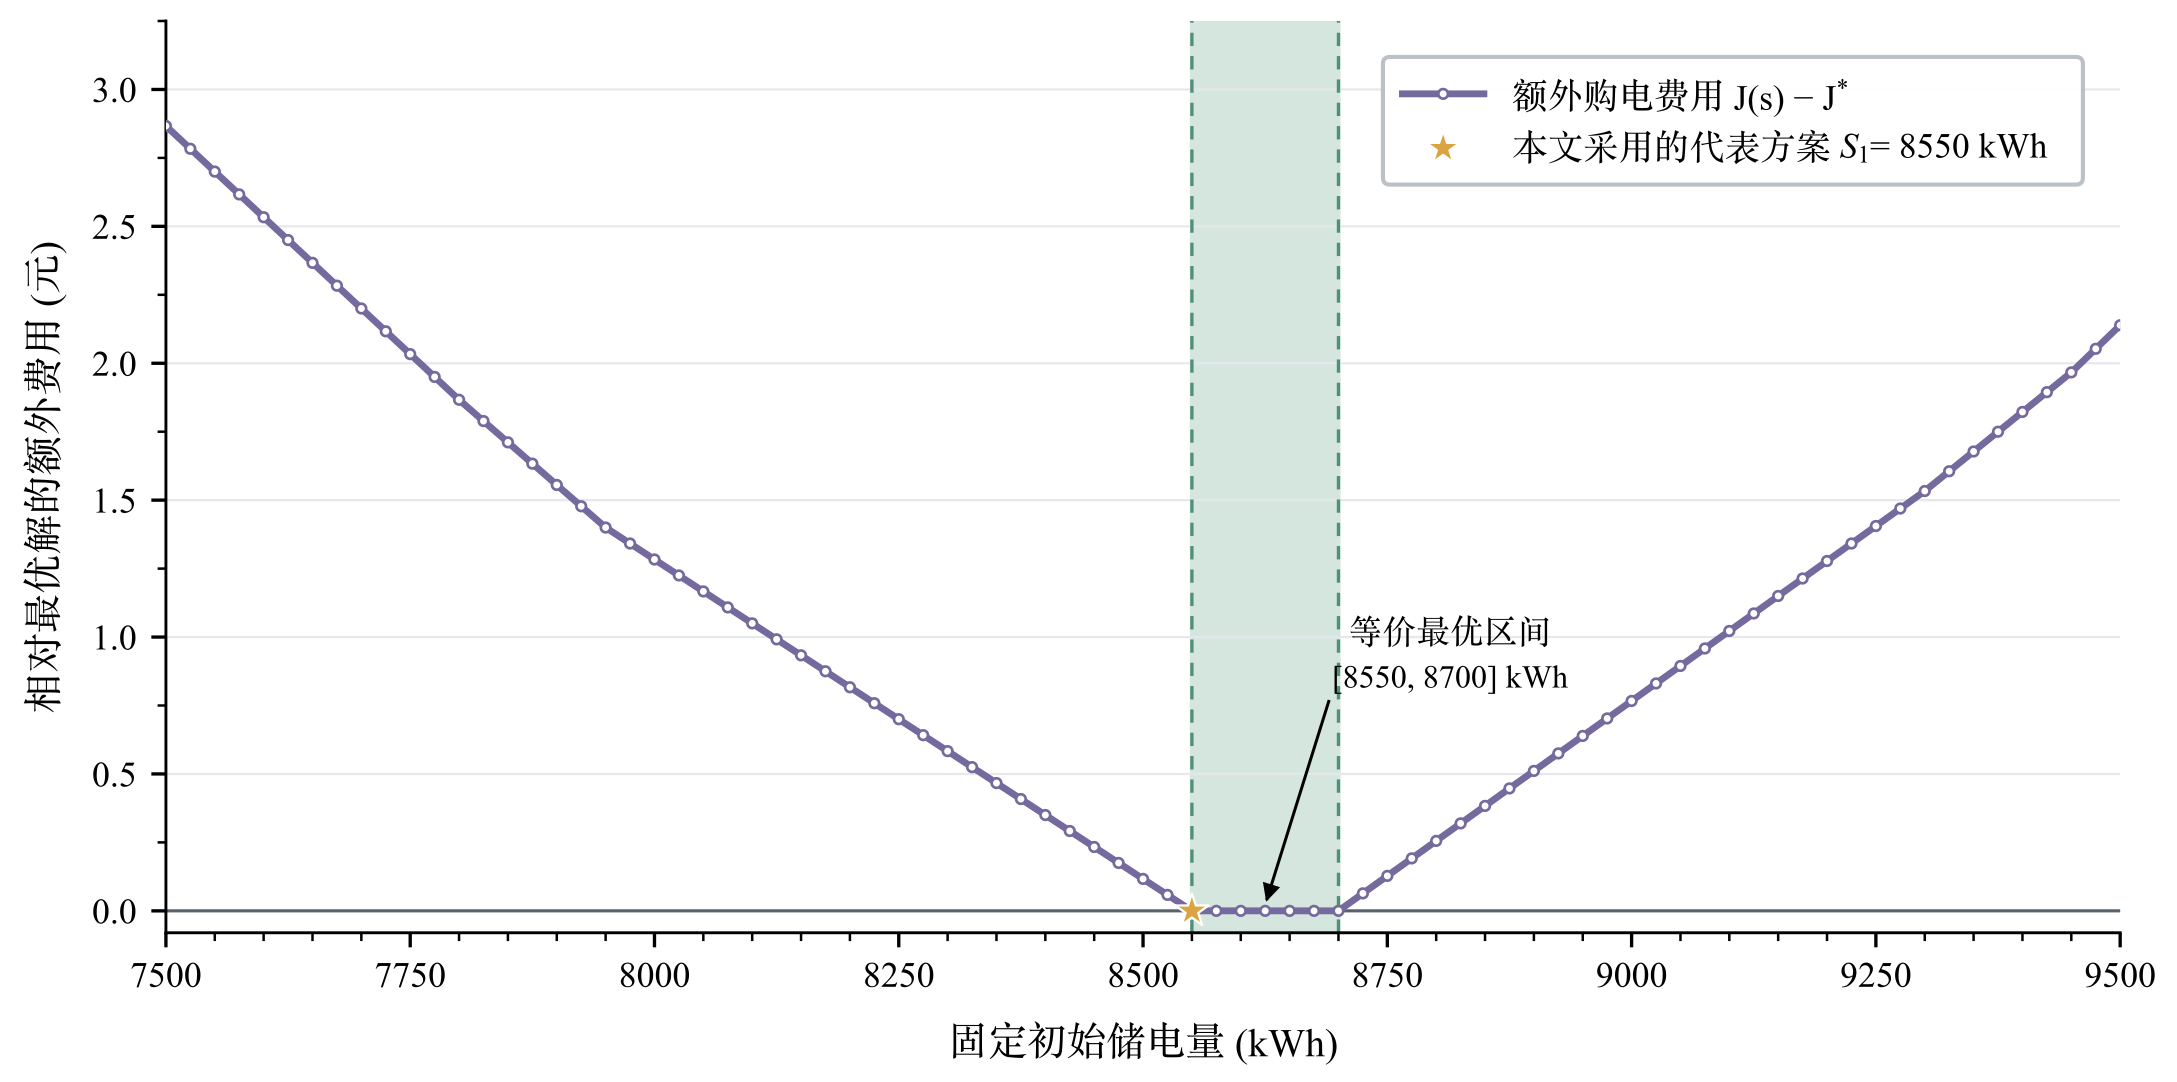
\includegraphics[width=0.66\textwidth]{figures/q1_s1_sensitivity.png}
  \caption{初始储电量对最优购电费用的局部影响}
  \label{fig:q1-s1-sensitivity}
\end{figure}

\subsection{结果分析}

题目指定的购电结果见表~\ref{tab:q1-grid}，最优方案全天购电 $59482.70\,\mathrm{kWh}$。

\begin{table}[!htbp]
  \centering
  \caption{问题一指定时段购电量及全天结果}
  \label{tab:q1-grid}
  \small
  \setlength{\tabcolsep}{4pt}
  \renewcommand{\arraystretch}{1.2}
  \begin{tabular}{crcrcr}
    \hline
    时间段 & 购电量/kWh & 时间段 & 购电量/kWh & 时间段 & 购电量/kWh \\
    \hline
    10:00--10:10 & 0.00 & 12:00--12:10 & 480.41 & 14:00--14:10 & 0.00 \\
    16:00--16:10 & 445.43 & 18:00--18:10 & 531.89 & 20:00--20:10 & 0.00 \\
    \multicolumn{2}{c}{全天购电量/kWh} & 59482.70 &
    \multicolumn{2}{c}{全天购电费/元} & 35118.60 \\
    \hline
  \end{tabular}
\end{table}

分时段充放电结果见表~\ref{tab:q1-storage}，调度轨迹见图~\ref{fig:q1-optimal-dispatch}。低价时段及午间光伏富余时，储能补充电量；早晚高价阶段则通过放电减少外网购电。日初与日末储电量均为 $8550.00\,\mathrm{kWh}$，运行范围为 $1200\sim10800\,\mathrm{kWh}$，且逐时段检查未发现同时充放电现象。可见，最优策略由电价、光伏出力和储能状态共同决定，不能仅按当期负载缺口安排购电。

\begin{table}[!htbp]
  \centering
  \caption{问题一储能设备分时段充放电量及日初日末储电量}
  \label{tab:q1-storage}
  \small
  \setlength{\tabcolsep}{4pt}
  \renewcommand{\arraystretch}{1.2}
  \begin{tabular}{crrcrr}
    \hline
    时间段 & 充电量/kWh & 放电量/kWh & 时间段 & 充电量/kWh & 放电量/kWh \\
    \hline
    00:00--04:00 & 1666.67 & 0.00 & 04:00--08:00 & 833.33 & 6365.84 \\
    08:00--12:00 & 4787.96 & 1703.00 & 12:00--16:00 & 5286.04 & 91.10 \\
    16:00--20:00 & 0.00 & 5780.13 & 20:00--24:00 & 8166.67 & 2859.87 \\
    \multicolumn{2}{c}{0:00 储电量/kWh} & 8550.00 &
    \multicolumn{2}{c}{24:00 储电量/kWh} & 8550.00 \\
    \hline
  \end{tabular}
\end{table}

\begin{figure}[!htbp]
  \centering
  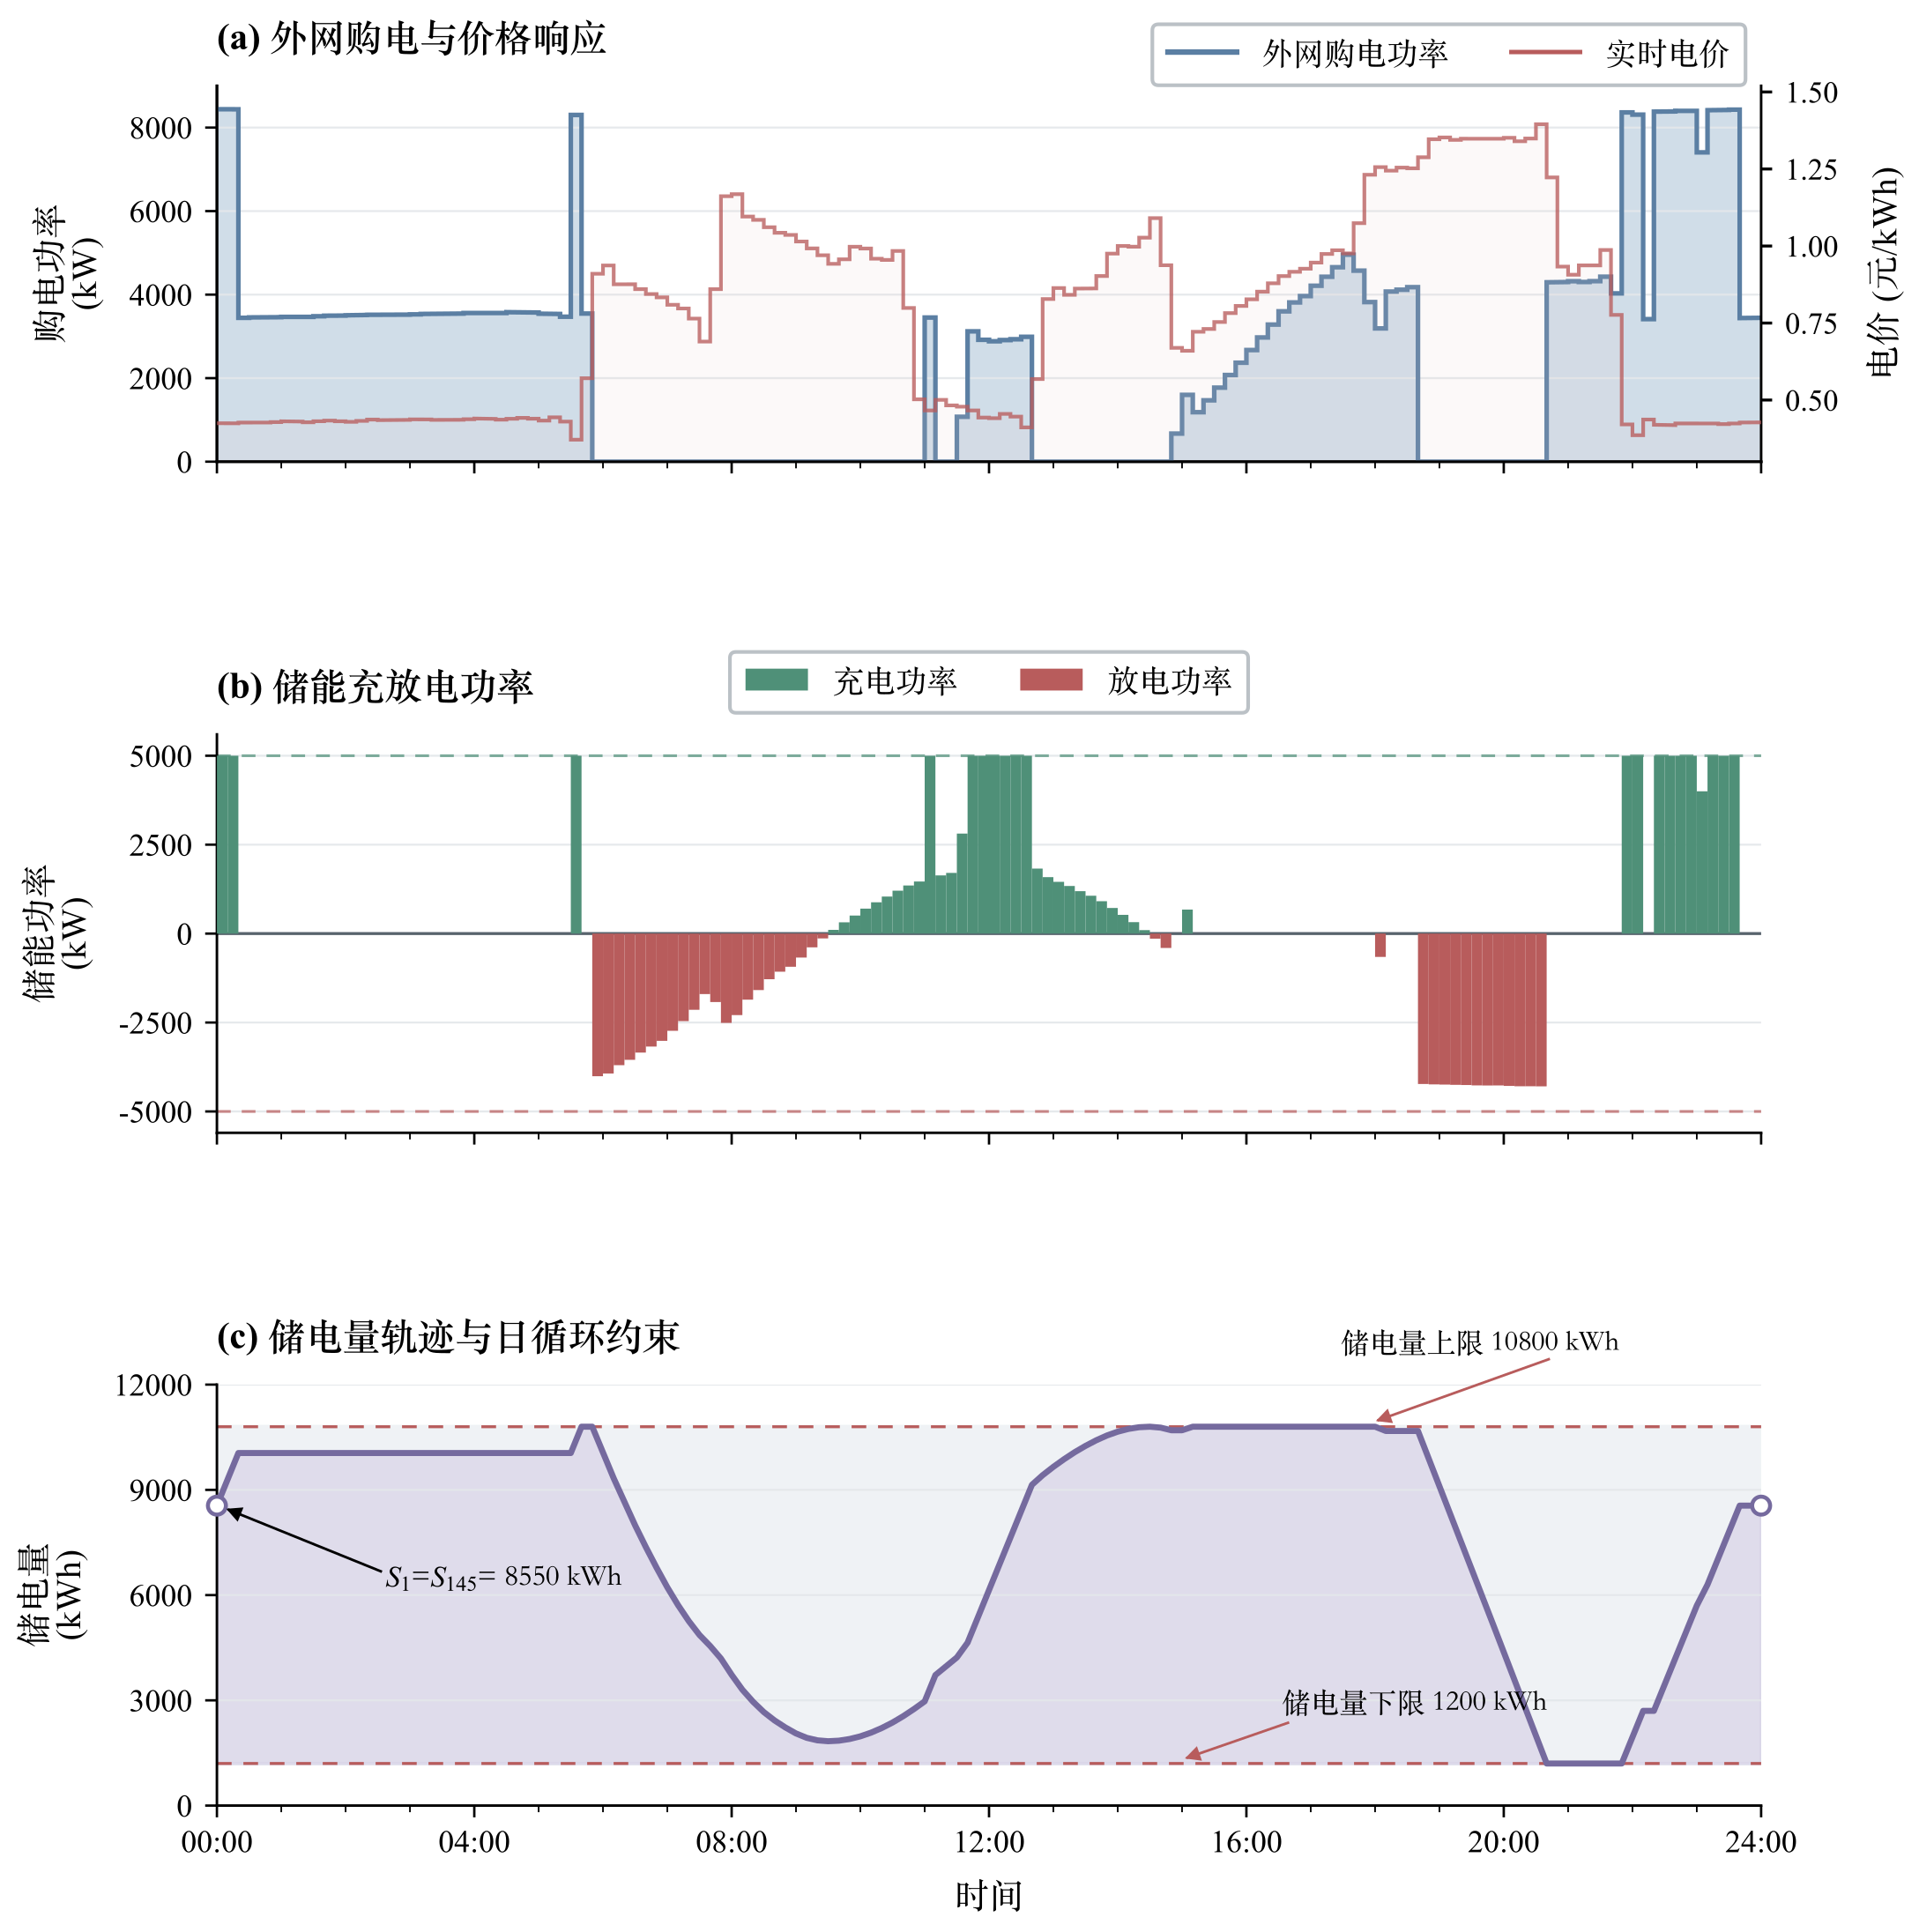
\includegraphics[width=0.55\textwidth]{figures/q1_optimal_dispatch.png}
  \caption{最优购电、储能充放电与储电量轨迹}
  \label{fig:q1-optimal-dispatch}
\end{figure}

为评价储能调度的经济效果，构造无储能基准方案：各时段优先利用光伏满足负载，不足部分由外网购电，富余光伏直接弃置。此时
\begin{equation}
  G_t^{0}=\max\{L_t-R_t,0\},\qquad
  J_0=\sum_{t=1}^{144}P_tG_t^{0}.
  \label{eq:q1-baseline}
\end{equation}

表~\ref{tab:q1-benefit} 显示，储能优化节省购电费用 $12933.45\,\text{元}$，节省率为 $26.92\%$，并将全天弃光量降为 0。图~\ref{fig:q1-cost-savings} 进一步表明，节费主要来自早晚高价阶段的放电，提前充电和日末补能则形成部分时段的额外支出。因此，储能调度应评价全天净收益：低价补能成本可由后续放电收益抵消，同时富余光伏也得以在本地消纳。

\begin{table}[!htbp]
  \centering
  \caption{问题一储能优化的经济效果}
  \label{tab:q1-benefit}
  \small
  \renewcommand{\arraystretch}{1.2}
  \begin{tabular}{lrrr}
    \hline
    指标 & 无储能基准 & 储能优化 & 变化量 \\
    \hline
    全天购电量/kWh & 61789.94 & 59482.70 & $-2307.24$ \\
    全天弃光量/kWh & 6247.96 & 0.00 & $-6247.96$ \\
    全天购电费用/元 & 48052.05 & 35118.60 & $-12933.45$ \\
    购电费用节省率 & --- & --- & $26.92\%$ \\
    \hline
  \end{tabular}
\end{table}

\begin{figure}[!htbp]
  \centering
  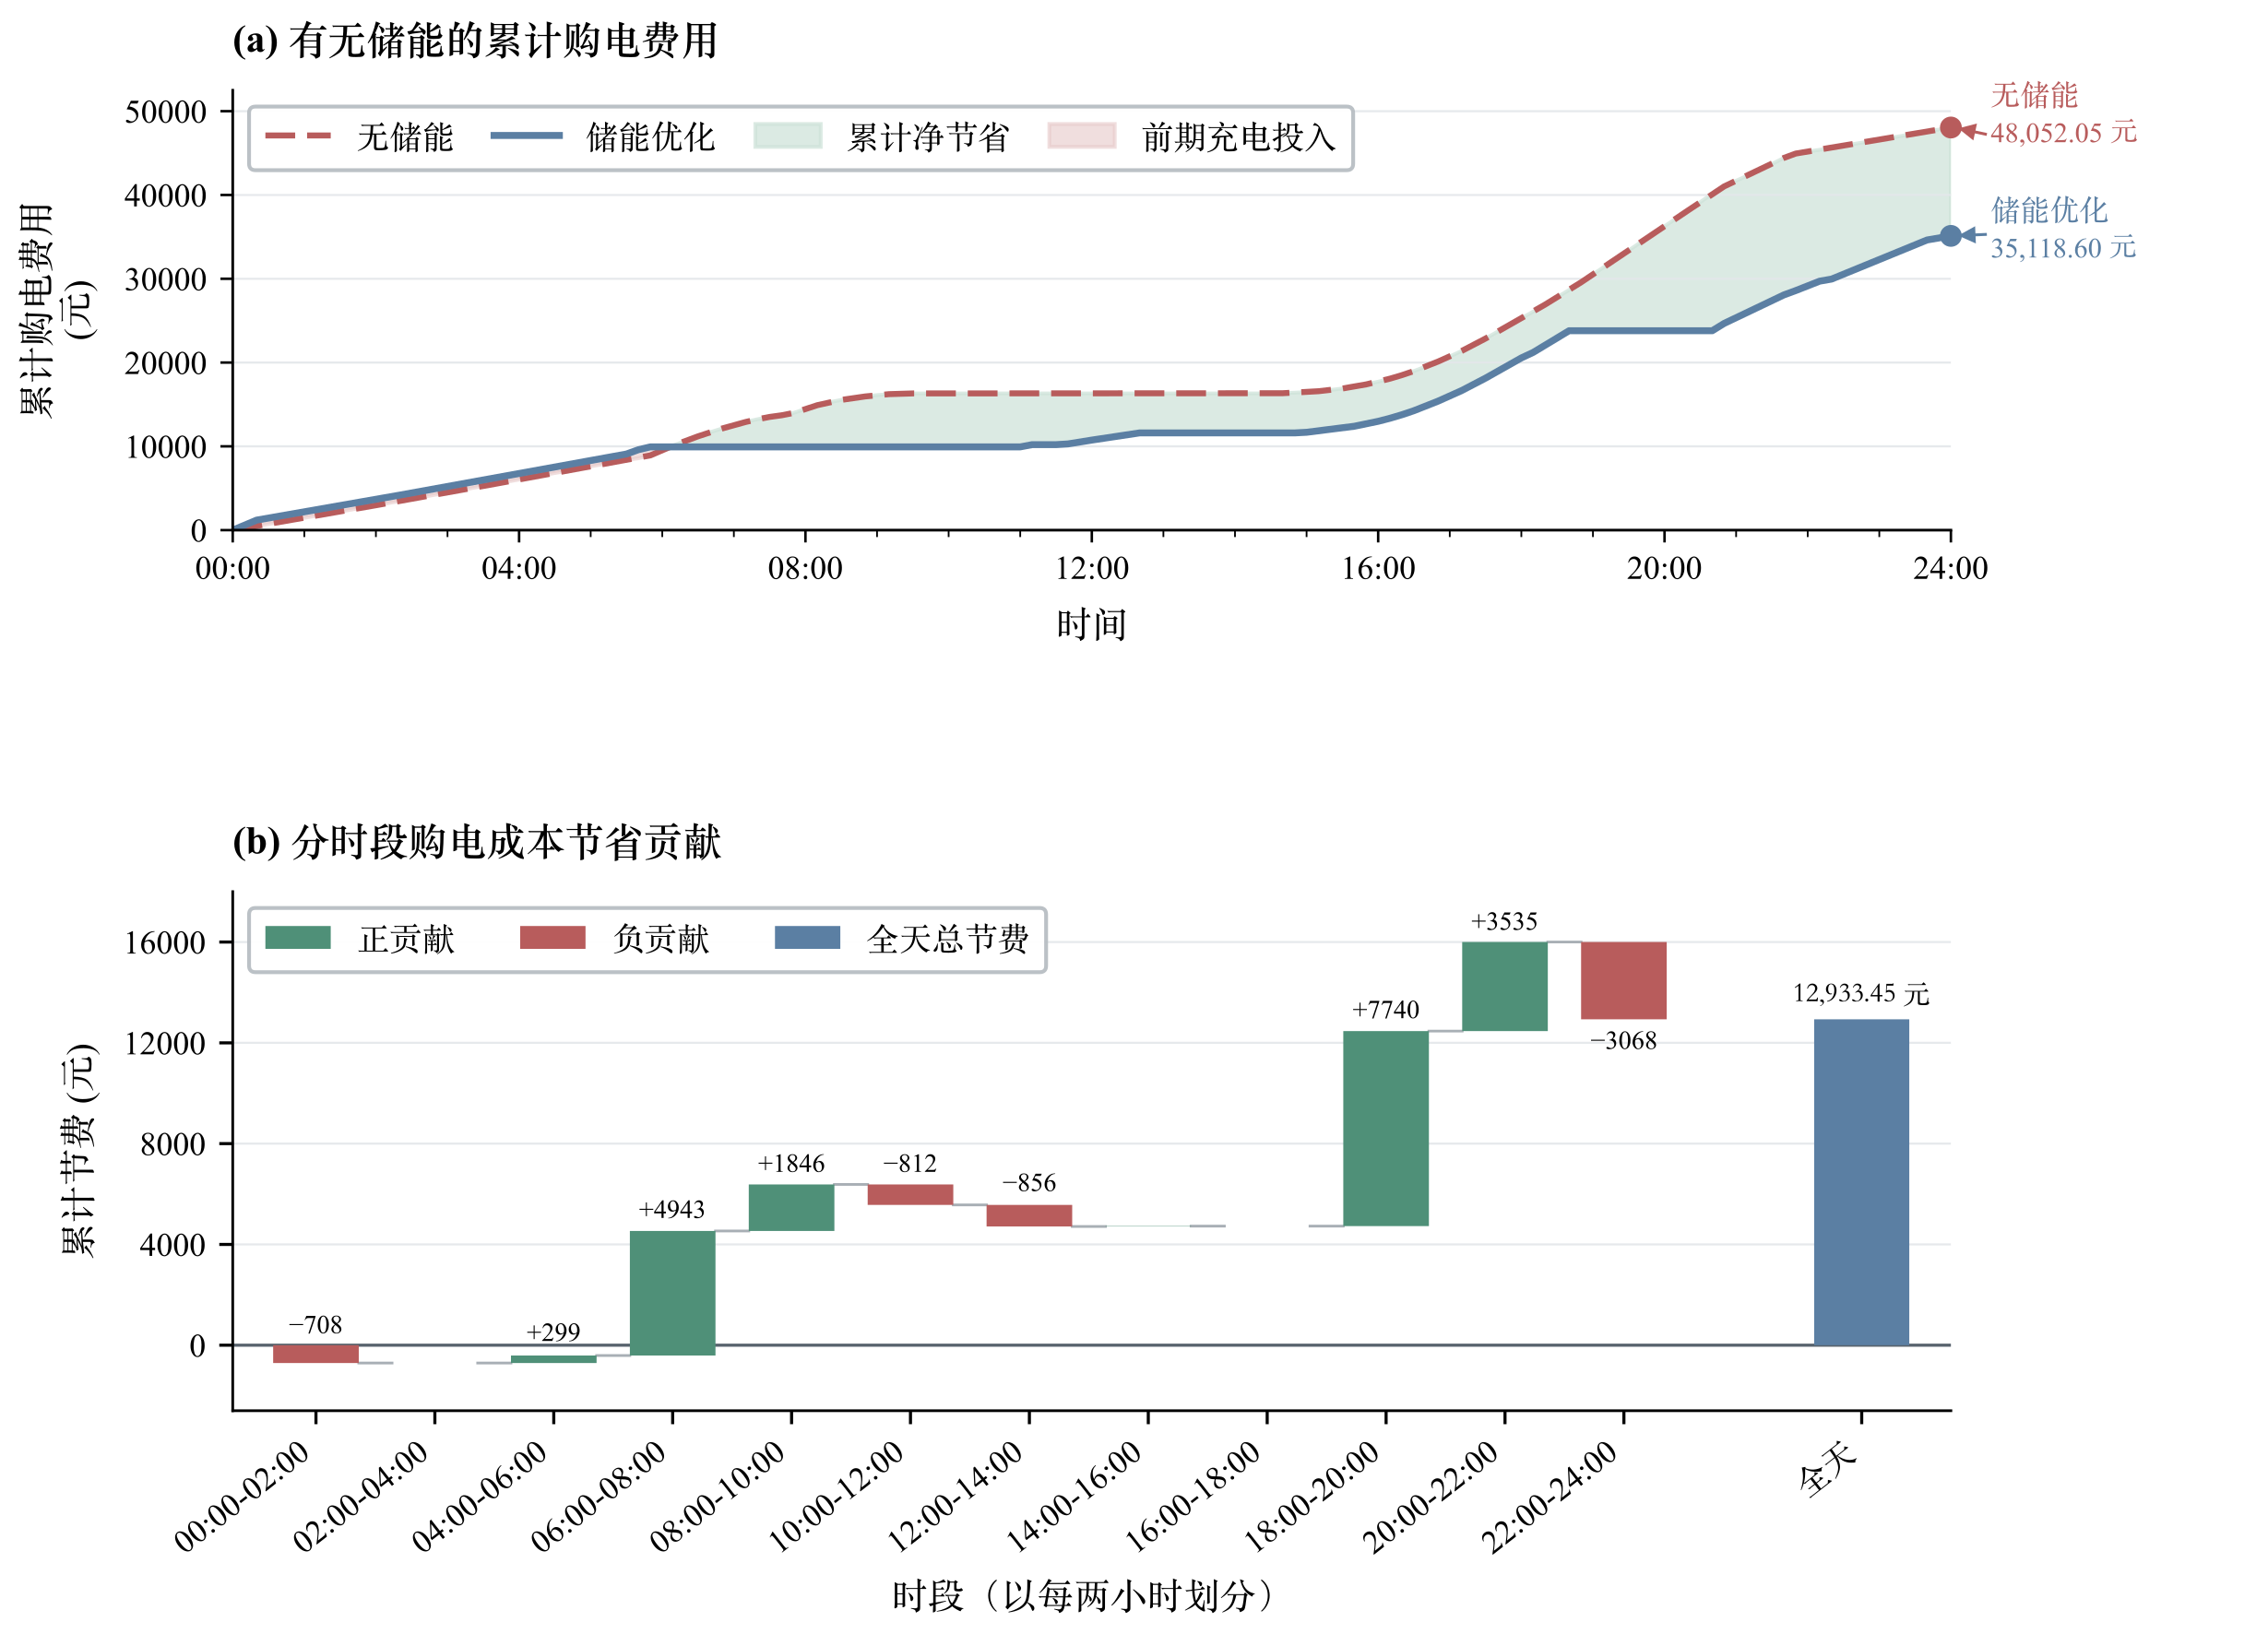
\includegraphics[width=0.70\textwidth]{figures/q1_cost_savings.png}
  \caption{有无储能的累计购电费用及分时段节费贡献}
  \label{fig:q1-cost-savings}
\end{figure}
